\section{Klassifikationsverfahren}\raggedbottom
Nachdem die Tweets vorbearbeitet, die Merkmale gewonnen und die Dimensionen zwecks verbesserter Performance reduziert wurden, können sie nun als Trainingsdatensatz für ein Klassifikationsverfahren verwendet werden. Im nachfolgenden Kapitel werden verschiedene solcher Verfahren vorgestellt und im Hinblick auf Voraussetzungen, Stärken und Schwächen analysiert. Ein besonderes Augenmerk soll in der Analyse auf jenen Parametern liegen, welche die Ergebnisse beim vorliegenden Datensatz maßgeblich beeinflussen können.    
\subsection{k-Nearest-Neighbor-Algorithmus}
Der k-Nearest-Neighbor-Algorithmus (KNN) ist eine parameterfreie Methode der Klassifikation \citep{Guo04}. Der zu klassifizierende Text wird zunächst analog zu den Trainingstexten vektorisiert. Über ein geeignetes Abstandsmaß werden nun die $k$ räumlich nächsten Nachbarn bestimmt. Der Text wird nun der Klasse zugeordnet, der die Mehrheit der Nachbarn angehören. Abbildung \ref{knn-alg} zeigt die k-Nearest-Neighbor-Klassifikation eines Punktes $x$ für $k=3$. Da die meisten Nachbarn hier dem Troll-Datensatz angehören, würde der zu $x$ gehörige Tweet somit als Troll-Tweet klassifiziert werden.\\
Die Wahl von $k$ ist entscheidend für die Qualität des Ergebnisses. Entscheidet man sich beispielsweise für ein zu kleines $k$, so ist möglich, dass vereinzelte Ausreißer die Genauigkeit trüben. Ist es auf der anderen Seite zu groß, so werden wahrscheinlich zu weit entfernte Punkte bei der Klassifikation miteinbezogen, was das Ergebnis wiederum verfälschen kann. Ferner ist bei Vorhandensein von 2 Klassen ein ungerades $k$ zu wählen, da andernfalls ein Unentschieden möglich ist.\\
\begin{figure}[htb]
	\begin{center}
		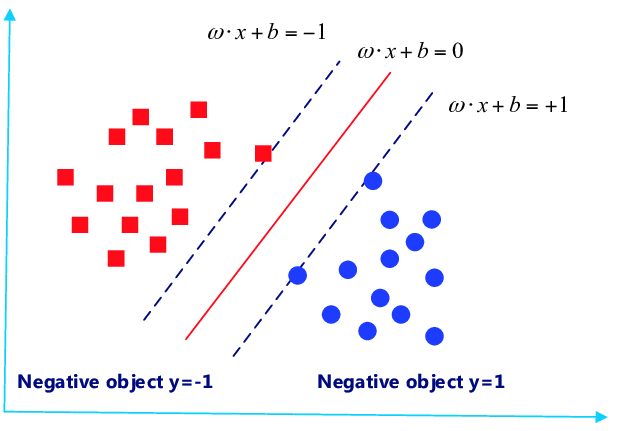
\includegraphics[scale=1.75]{bilder/Abb4.png}
		\caption{KNN-Klassifizierung für $k=3$}\label{knn-alg}
	\end{center}
\end{figure}\\
Eine zwingende Voraussetzung, um zuverlässig mit dem KNN-Algorithmus in diesem Projekt arbeiten zu können, ist die Dimensionalitätsreduktion. Die Merkmalsextraktion bringt bei den mehr als 600.000 Tweets hochdimensionale Vektoren hervor. Unbehandelt wären aufgrund der komponentenweisen Abstandsmessung Laufzeiten von einigen Minuten zu erwarten.\\
Die Vorteile dieses Verfahrens sind die einfache Implementierung und seine Eignung für alle möglichen Ausprägungen von Merkmalsräumen. Als Schwächen werden die bereits angesprochenen Probleme mit der Performance angesehen.
\subsection{Naiver Bayes-Klassifikator}
Der Naive Bayes-Klassifikator (NB) ist ein statistisches Verfahren der Klassifikation \citep{Rish01}. Die Grundlage der Berechnung bildet hier der Satz von Bayes, bekannt aus der Wahrscheinlichkeitstheorie. In seiner herkömmlichen Interpretation beschreibt dieser die Berechnung der Wahrscheinlichkeit, dass ein Ereignis dem anderen vorausgegangen ist. Wendet man dies auf einen gegebenen Text $t \in T$ und die Klasse $k_i \in K$ an, so erhält man die Formel für die Wahrscheinlichkeit, dass $t$ der Klasse $k_i$ angehört (siehe Gleichung \ref{bayes}).
\begin{equation}
	P(k_i|t) = \frac{P(t|k_i) \cdot P(k_i)}{P(t)}
	\label{bayes}
\end{equation}
Der Klassifikator bestimmt nun diejenige Klasse $k_i$, für die der Wert dieser Formel maximal ist. Mathematisch formuliert:
\begin{equation}
	k = arg \max\limits_{k_i \in K} P(k_i|t) = arg \max\limits_{k_i \in K} \frac{P(t|k_i) \cdot P(k_i)}{P(t)}
\end{equation}
Die Werte für $P(k_i)$ und $P(t)$ werden a priori über relative Anteilshäufigkeiten, also über den Anteil einer Klasse und den Anteil eines Textes am gesamten Merkmalraum, bestimmt. Für die Maximierung wird meist die Maximum-Likelihood-Methode benutzt.\\
Jeder Klasse wird vor der Klassifizierung eine bestimmte Form der Wahrscheinlichkeitsverteilung, meist eine Normalverteilung, und die stochastische Unabhängigkeit der Merkmale unterstellt. Letztere Annahme ist \glqq naiv\grqq{}  weil nicht immer zutreffend, der Algorithmus liefert in der Praxis bei vielen Anwendungen dennoch solide Ergebnisse. Wird diese Annahme hingegen durch stark korrelierte Daten gröber verletzt, so sind Genauigkeitsverluste zu erwarten, was eine Schwäche dieses Verfahrens ist. Im Rahmen der Evaluation werden Ergebnisse unter Annahme einer Normalverteilung und einer Multinomialverteilung verglichen.
\pagebreak
\subsection{Support Vector Machine}
Ein anderes Lernmodell trägt den Namen Support Vector Machine (SVM) \citep{Nayak15}. Die Grundidee ist hier, die vorliegenden Klassen im multidimensionalen Raum durch Einschub einer Hyperebene räumlich zu trennen. Die Ebene wird dabei so platziert, dass der Abstand zu den nächstliegenden Vektoren der beiden Klassen, den sogenannten Stützvektoren (engl. \textit{support vectors}) maximal ist. Abbildung \ref{svm-alg} zeigt beispielhaft zwei solcher durch eine Hyperebene (rote Gerade) getrennte Klassen in einem zweidimensionalen Merkmalraum. 
\begin{figure}[htb]
	\begin{center}
		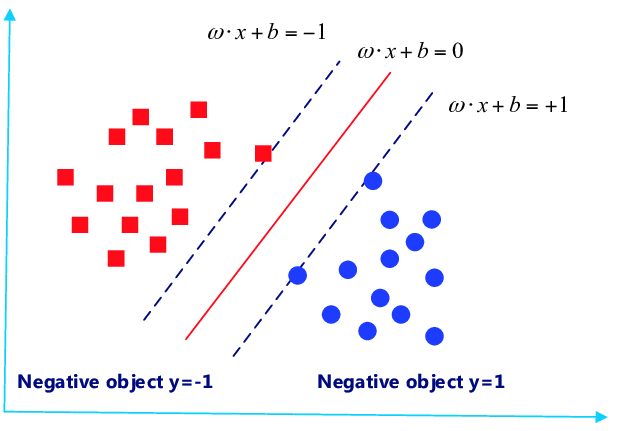
\includegraphics[scale=0.75]{bilder/Abb5.png}
		\caption{SVM-Klassifizierung \citep{Zhou16}}\label{svm-alg}
	\end{center}
\end{figure}\\
 Für ein zu klassifizierendes Objekt wird nun mithilfe einer Entscheidungsfunktion festgestellt, auf welcher Seite der Ebene es liegt und kann so eindeutig einer Klasse zugeordnet werden. Ist der Einschub einer Hyperebene nicht möglich, d.h. sind die Klassen nicht linear trennbar, so behilft man sich mit dem sogenannten \glqq Kernel-Trick\grqq{}: Der Merkmalraum wird auf einen höherdimensionalen Raum abgebildet, in welchem die Klassen dann linear trennbar sind. Diese Transformation benötigt eine hohe Rechenleistung und stellt deshalb bei stark überlappenden Klassen eine Schwäche dieses Verfahrens dar. Bei weniger überlappenden oder linear trennbaren Klassen ist der Algorithmus in der Einstufung jedoch sehr schnell. Ein weiterer Vorteil ist der relativ geringe Speicherverbrauch, da zur Klassifikation nur ein Teil der Trainingsdaten gebraucht wird.\\
 Zwei Parameter, die die Ergebnisse beeinflussen können, sind zum einen der Bestrafungsparameter $C$ und der Gamma-Wert. $C$ gibt an, wie stark die Gefahr der Falschklassifizierung berücksichtigt werden soll. Je niedriger der Wert, desto leichter wird es, eine Trennung zu vollziehen und dabei einzelne Ausreißer zu ignorieren. Allerdings findet dann bei mäßiger bis starker Überlappung keine eindeutige Trennung der Klassen statt. Je höher der Wert, desto strenger versucht der Algorithmus, alle Punkte in der Entscheidung miteinzubeziehen. Hier besteht die Gefahr der Überanpassung. Der Gamma-Wert gibt an, wie stark einzelne Punkte beim Kernel-Trick Einfluss auf die Gruppierung haben, also wie granular die Gruppen sind. Bei linear trennbaren Klassen kommt er demnach nicht zur Anwendung. Um zu guten Ergebnissen zu kommen, ist eine gute Balance der beiden Werte, in jedem Fall aber die Anpassung an den Datensatz von Nöten.
\subsection{Entscheidungsbäume}
Die Grundlage für ein weiteres Klassifikationsverfahren sind die sogenannten Entscheidungsbäume (engl. \textit{decision trees}) (\textcolor{red}{Quelle}). Hierbei handelt es sich um herkömmliche, aus der Graphentheorie bekannte Bäume, welche eine Entscheidungsfolge abbilden. Für jedes zu klassifizierende Objekt wird der Baum einmal durchlaufen. An jedem inneren Knoten wird nun der Wert eines extrahierten Merkmals abgefragt. Je nach Ergebnis des Vergleichs wird entschieden, welches Kind als nächstes besucht wird. Die Blätter beinhalten die möglichen Klassen, sodass nach der letzten Entscheidung mit Ankommen am Ende des Baumes die Klassifikation vollzogen ist. Abbildung \ref{dtree} zeigt beispielhaft einen Entscheidungsbaum für die Klassifikation eines Messestandorts anhand von drei Merkmalen. Die möglichen Klassen für einen Standort sind \glqq geeignet\grqq{} und \glqq ungeeignet\grqq{}.
\begin{figure}[htb]
	\begin{center}
		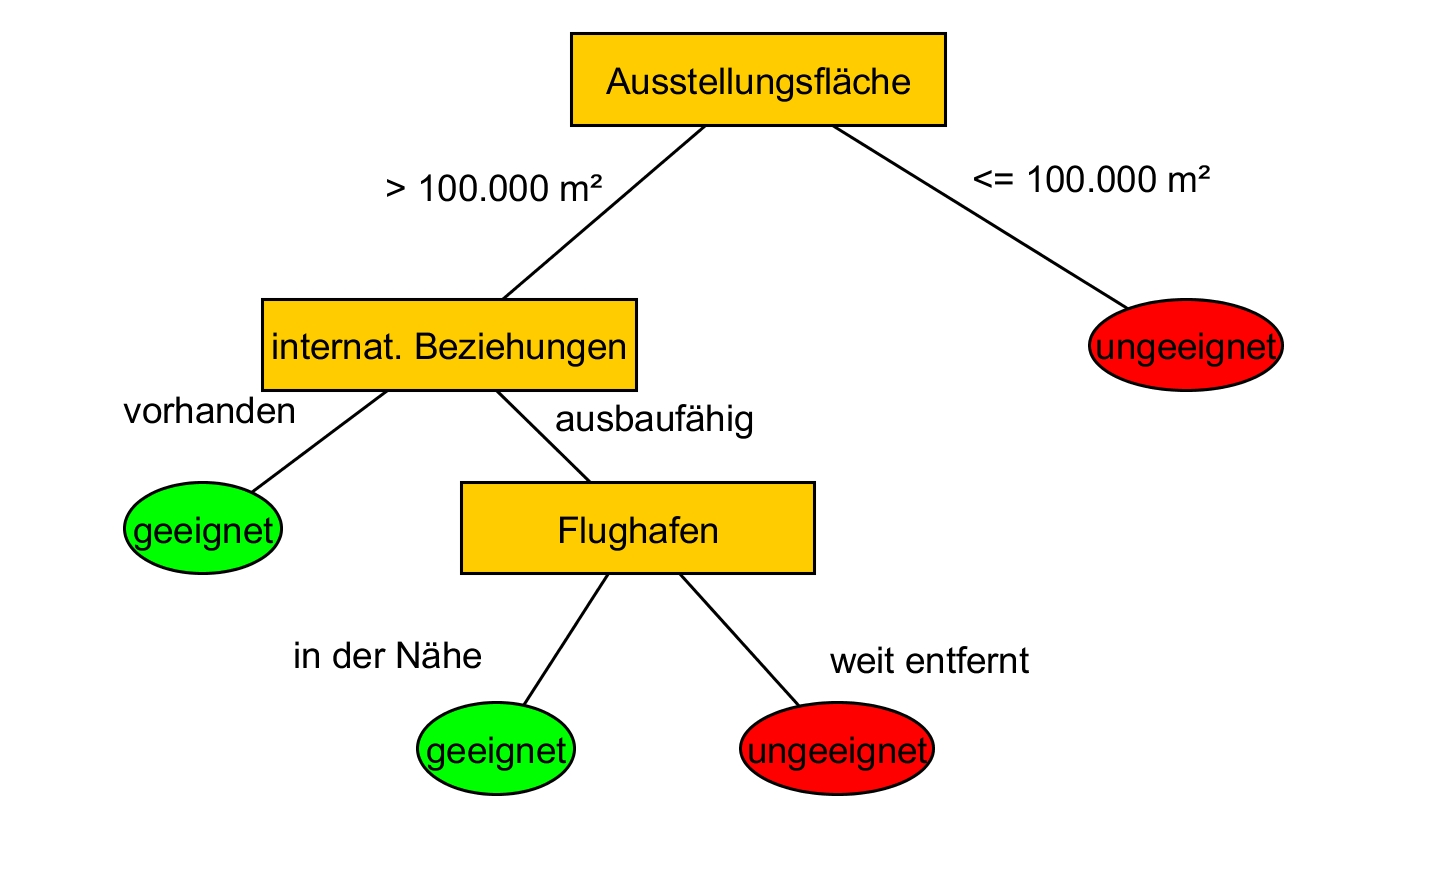
\includegraphics[scale=0.25]{bilder/Abb6.jpg}
		\caption{Entscheidungsbaum zur Klassifizierung eines Messestandorts}\label{dtree}
	\end{center}
\end{figure}\\
Das Training bzw. das Lernen besteht bei diesem Verfahren im Aufbau des Baumes. Beginnend bei der Wurzel wird nun dasjenige Merkmal bestimmt, welches den größten Fortschritt in der Klassifikationsentscheidung bringt. Ein gebräuchliches Maß dafür ist die \textit{Gini Impurity}, welche die Homogenität bzw. Heterogenität der Daten anzeigt. Gleichsam anwendbar ist hier auch die Entropie, welche den mittleren Informationsgehalt des Merkmalvektors misst. Das gefundene Merkmal dient nun zur Aufteilung der ursprünglichen Datenmenge. Auf die neu entstehenden Mengen wird diese Methode nun rekursiv angewendet bis Mengen erzeugt werden, deren Elemente alle der gleichen Klasse angehören.\\
Durch die klare Strukturierung und grafische Darstellbarkeit ist die Entscheidungsbaum-Klassifikation als Konzept leicht verständlich. Ein weiterer Vorteil ist eine automatische Merkmalfilterung beim Aufbau des Baums: Merkmale, die durch Gini Impurity bzw. Entropie als irrelevant erkannt wurden, können leicht weggelassen werden. Hier sind Zeit- und Speichergewinne möglich.\\
Eine Schwäche dieses Verfahrens ist die schwache Robustheit der Entscheidungsbäume. Dies bedeutet, dass kleine Änderungen im Ausgangsdatensatz zu sehr großen Veränderungen in der Datenstruktur und der anschließenden Klassifikation führen können.
\subsection{Mehrschichtiges Perzeptron}
Das mehrschichtige Perzeptron (engl. \textit{multi-layer perceptron, MLP}) ist ein Vertreter der künstlichen neuronalen Netze (\textcolor{red}{Quelle}). In seinem grundlegenden Aufbau ähnelt es einem Logikgatter. Die grundlegenden Bausteine, analog zu Gehirnzellen Neuronen genannt, sind in Schichten angeordnet. Die Eingabeschicht nimmt den Merkmalvektor komponentenweise entgegen, während die Neuronen der Ausgabeschicht das Klassifikationsergebnis ausgeben. Die dazwischenliegenden Schichten werden versteckte Schichten bzw. \textit{hidden layers} genannt. Abbildung \ref{mlp-ex} illustiert ein Beispiel für Netz, welches einen vierdimensionalen Vektor verarbeitet.\\
 \begin{figure}[htb]
	\begin{center}
		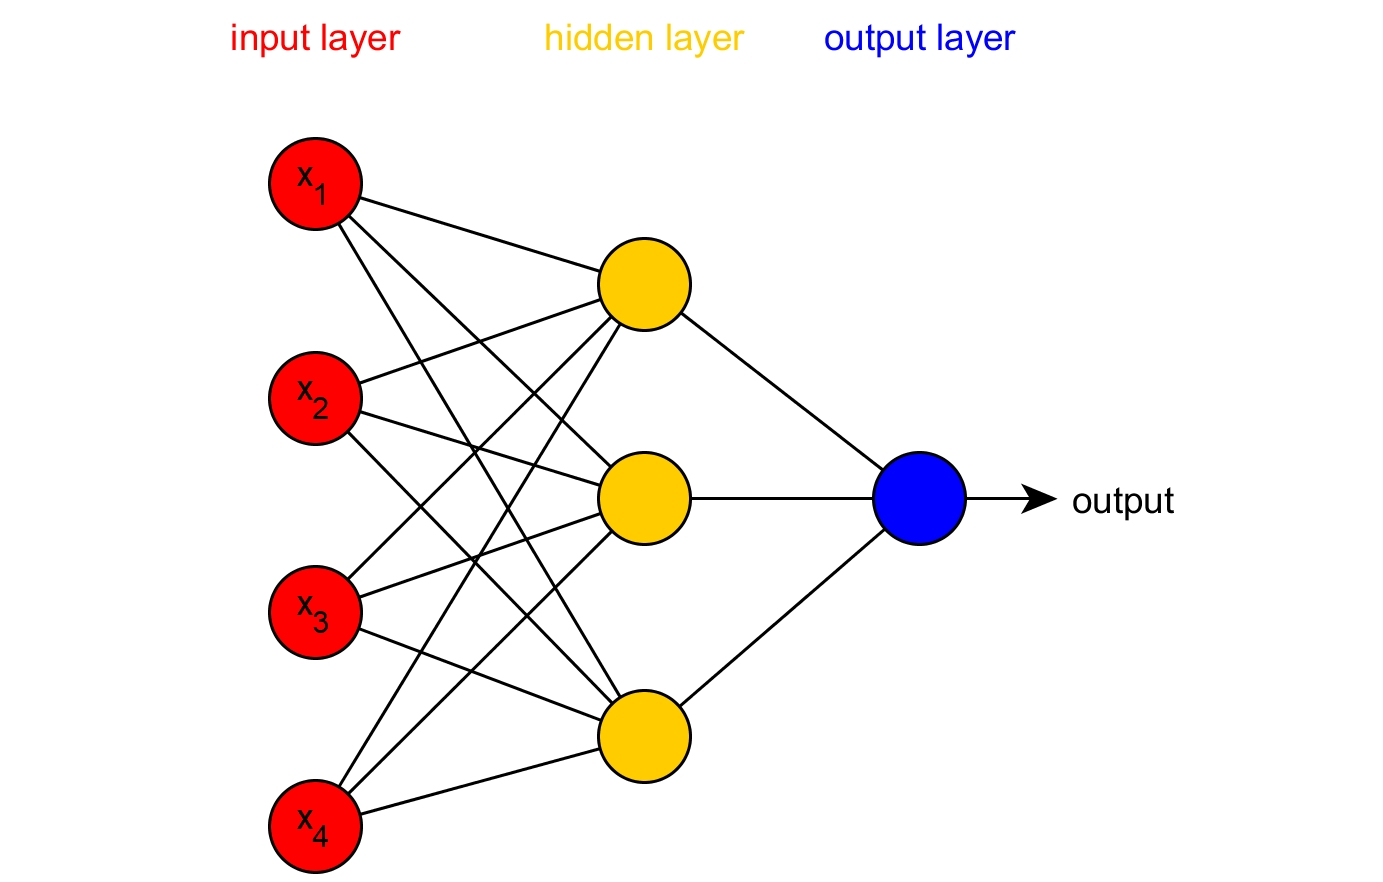
\includegraphics[scale=0.20]{bilder/Abb7.jpg}
		\caption{Beispiel für mehrschichtiges Perzeptron}\label{mlp-ex}
	\end{center}
\end{figure}\\
Jedes Neuron einer Schicht hat eine Verbindung, ähnlich einer Kante, zu einem Neuron (oft auch zu allen) der nächsten Schicht. Die Verbindung trägt ein Gewicht. Dazu trägt auch jedes Neuron einer versteckten Schicht und der Output-Schicht ein sogenanntes Verzerrungsgewicht bzw. \textit{bias weight} $b$.\\
 Der Lernprozess läuft nun wie folgt ab: Beginnend bei den Input-Neuronen wird für jede Eingabe eine gegebene Aktivierungsfunktion berechnet. Das Ergebnis wird an die nachfolgenden Neuronen weitergeschickt und erneut die Aktivierungsfunktion berechnet. Ist es schließlich in der Output-Schicht angekommen, so wird das Ergebnis interpretiert und mit der vorher deklarierten Klasse verglichen. Ist das Ergebnis falsch, so werden die Gewichte des Netzes von hinten nach vorne neujustiert. Man spricht hier von \textit{Backpropagation}. Auf diese Weise lernt das Netz mit jedem Fehler dazu und die Klassifikation wird zunehmend genauer.
\pagebreak